\chapter{时序分析与电路优化}
本章节主要对第二章设计的电路图导出.cdl网表借助HSpice工具软件进行时序分析,即输入到输出延时的大小的检测。
\section{工具简介}
HSPICE 是Meta-Software 公司为集成电路设计中的稳态分析,瞬态分析和频域分析等电路性能的模拟分析而开发的一个商业化通用电路模拟程序,它在伯克利的SPICE(1972 年推出),MicroSim公司的PSPICE (1984 年推出)以及其它电路分析软件的基础上,又加入了一些新的功能,经过不断的改进,目前已被许多公司、大学和研究开发机构广泛应用。

HSPICE 可与许多主要的EDA 设计工具,诸如Cadence,Workview 等兼容,能提供许多重要的针对集成电路性能的电路仿真和设计结果。采用HSPICE 软件可以在直流到高于100GHz 的微波频率范围内对电路作精确的仿真、分析和优化。在实际应用中, HSPICE能提供关键性的电路模拟和设计方案,并且应用HSPICE进行电路模拟时,其电路规模仅取决于用户计算机的实际存储器容量。

本次实验中需要对网表进行修改,相关原理主要参考文献\cite{bookHSpice2007},电子书版权为复旦大学所有。

\section{基于HSpice的时序结果}
在由Composer导出NORM模块的网表后,需要在网表中添加工艺库以及激励等信息,这两部分信息如下所示,首先确定.13的工艺库以及温度等参数。
\begin{verbatim}
0.13um INV Characteristics
.options LIST NODE POST
.lib 'l013_v2p5.lib' TT
.TEMP 25
.GLOBAL VDD, GND
OP
\end{verbatim}
下面是网表中输入的激励:
\begin{verbatim}
X Lzc<31> Lzc<30> Lzc<29> Lzc<28> Lzc<27> Lzc<26> Lzc<25>
+Lzc<24> Lzc<23> Lzc<22> Lzc<21> Lzc<20> Lzc<19> Lzc<18> Lzc<17> Lzc<16>
+Lzc<15> Lzc<14> Lzc<13> Lzc<12> Lzc<11> Lzc<10> Lzc<9> Lzc<8> Lzc<7> Lzc<6>
+Lzc<5> Lzc<4> Lzc<3> Lzc<2> Lzc<1> Lzc<0> Src<31> src1<30> src1<29>
+Src<28> Src<27> Src<26> Src<25> Src<24> Src<23> Src<22> Src<21>
+Src<20> Src<19> Src<18> Src<17> Src<16> Src<15> Src<14> Src<13>
+Src<12> Src<11> Src<10> Src<9> Src<8> Src<7> Src<6> Src<5> Src<4>
+Src<3> Src<2> Src<1> Src<0> 
+NORM
V1 VDD 0 1.2V
V4 Src<31> 0 0
V5 Src<30> 0 0
V6 Src<29> 0 0
V7 Src<28> 0 pulse(0 1.2V 0.5N 0N 0N 2N 4N) 
V8 Src<27> 0 1.2V
V9 Src<26> 0 1.2V 
V10 Src<25> 0 1.2V 
V11 Src<24> 0 1.2V 
V12 Src<23> 0 0
V13 Src<22> 0 0
V14 Src<21> 0 0 
V15 Src<20> 0 0
V16 Src<19> 0 0
V17 Src<18> 0 0 
V18 Src<17> 0 0 
V19 Src<16> 0 0 
V20 Src<15> 0 0
V21 Src<14> 0 0
V22 Src<13> 0 0
V23 Src<12> 0 0
V24 Src<11> 0 1.2V
V25 Src<10> 0 0
V26 Src<9> 0 1.2V 
V27 Src<8> 0 1.2V 
V28 Src<7> 0 1.2V 
V29 Src<6> 0 1.2V 
V30 Src<5> 0 1.2V 
V31 Src<4> 0 1.2V 
V32 Src<3> 0 1.2V 
V33 Src<2> 0 1.2V
V34 Src<1> 0 1.2V 
V35 Src<0> 0 1.2V
.tran 0.2n 10n
.end
\end{verbatim}
根据NORM指令的具体功能,在输入端口Src<28>输入周期为4ns的脉冲瞬态电压源,脉冲宽度为2ns。定义电压脉冲源的具体语法如下所示:
\begin{verbatim}
Vxxx n+ n- PU<LSE> <(>v1 v2 <td <tr <tf <pw <per>>>>>  <)>
\end{verbatim}
其中\verb|< >|为可省略部分。.trans 0.2n 10n表示工具共需要分析10ns的瞬态分析,步长为0.2ns。

最后,HSpice的时序分析结果如图\ref{fig4.1}所示。从图中可以看出,当输入为最高5位(包括符号位)由00001变为00011时,输出的最低两位由11变为10,其输出延时为395ps(如图所示),同时,输出随输入的变化情况与NC的仿真波形都说明设计的NORM指令模块功能的正确性!
\begin{figure}[!hbtp]
\centering
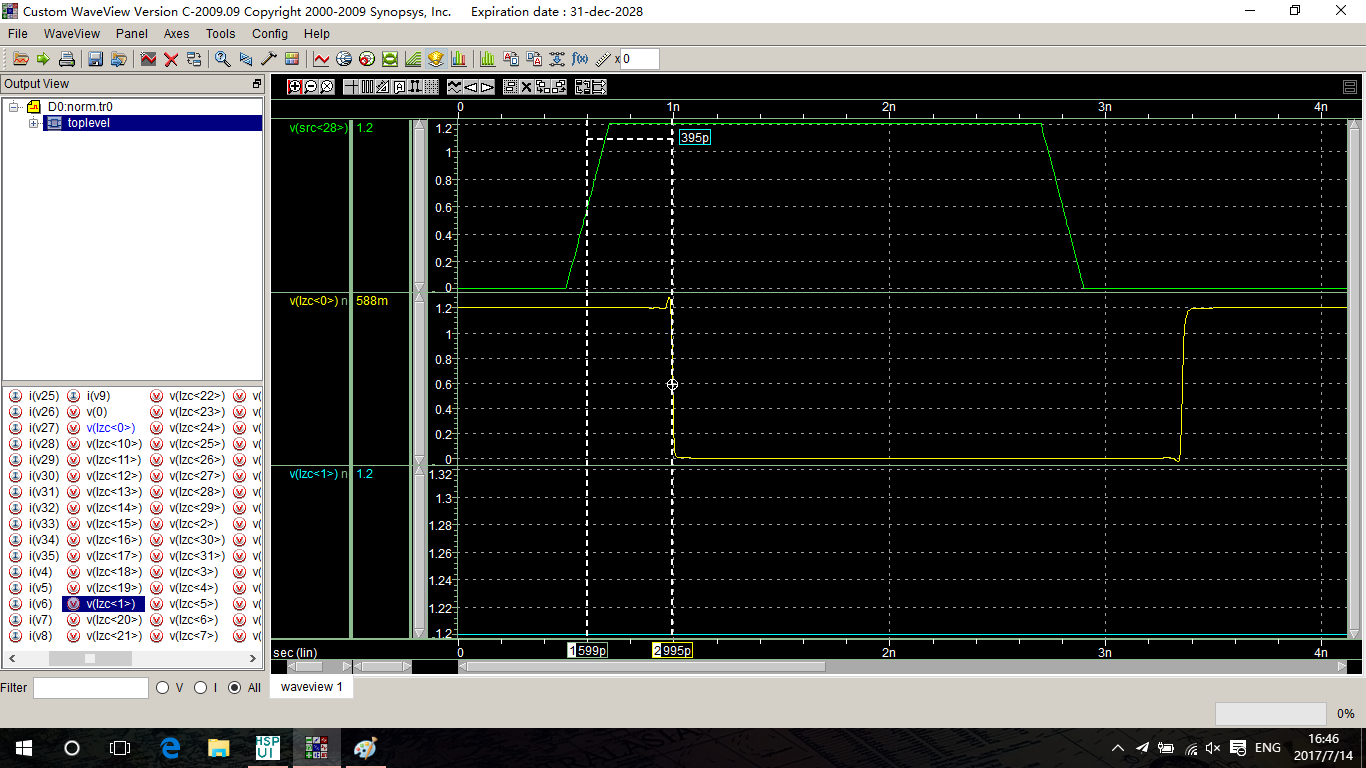
\includegraphics[width=0.9\textwidth]{chapter4/NORM_HSPICE_1}
\caption{NORM指令的HSpice分析结果}
\label{fig4.1}
\end{figure}
